\section{Results}

Before the behaviour of the algorithms is analysed, some plots of kinematic variables are shown
in Fig.~\ref{fig:kinematics}.
It can be seen that the algorithms do not greatly differ on the kinematics of the events.
In particular, \spectral{} clustering does not appear to sculpt any distributions in any of the datasets involving Higgs bosons and top (anti)quarks.


\begin{figure}[htp]
    \begin{center}
    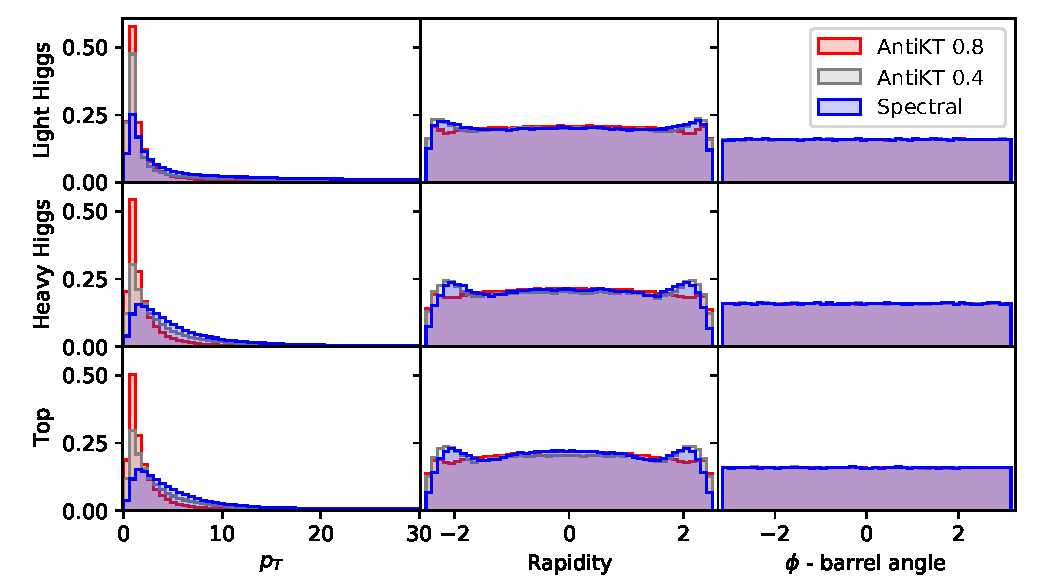
\includegraphics[width=\textwidth]{graphics/kinematics}
        \caption{Basic jet variables for each of the analysis datasets and three clustering algorithms.
            In the first column there are some noticeable differences in the transverse momentum.
            In the second column the rapidity shows that
            the algorithms cluster jets at the edge of the barrel slightly differently.
            In the third column the barrel angle shows no noticeable changes.
        }\label{fig:kinematics}
\end{center}
\end{figure}

\subsection{IR safety}
Shape variables (see the QCD section of Ref.~\cite{Altarelli:1989hv} for a useful review), such as jet mass, thrust, sphericity, spherocity and oblateness,  are sensitive to IR divergences.
For each configuration of the clustering algorithm we expect an IR safe algorithm to present a stable transition
in a shape variable from the LO to NLO datasets, as significant
changes in the spectra would indicate sensitivity to soft and collinear radiation.
The clustering and evaluation here is done using the \underline{3-jets} dataset, as described in section~\ref{sec:particle_data}.
Shape variables are calculated from the total momentum of the 4 jets with highest \(p_T\) in each event.
This comparison is made in Fig.~\ref{fig:IRC_singles2}.
It can be seen in this figure that little difference exists between \genkt{} and \spectral{} clustering, so as to reinforce that they are both IR safe.

\begin{figure}[htp]
    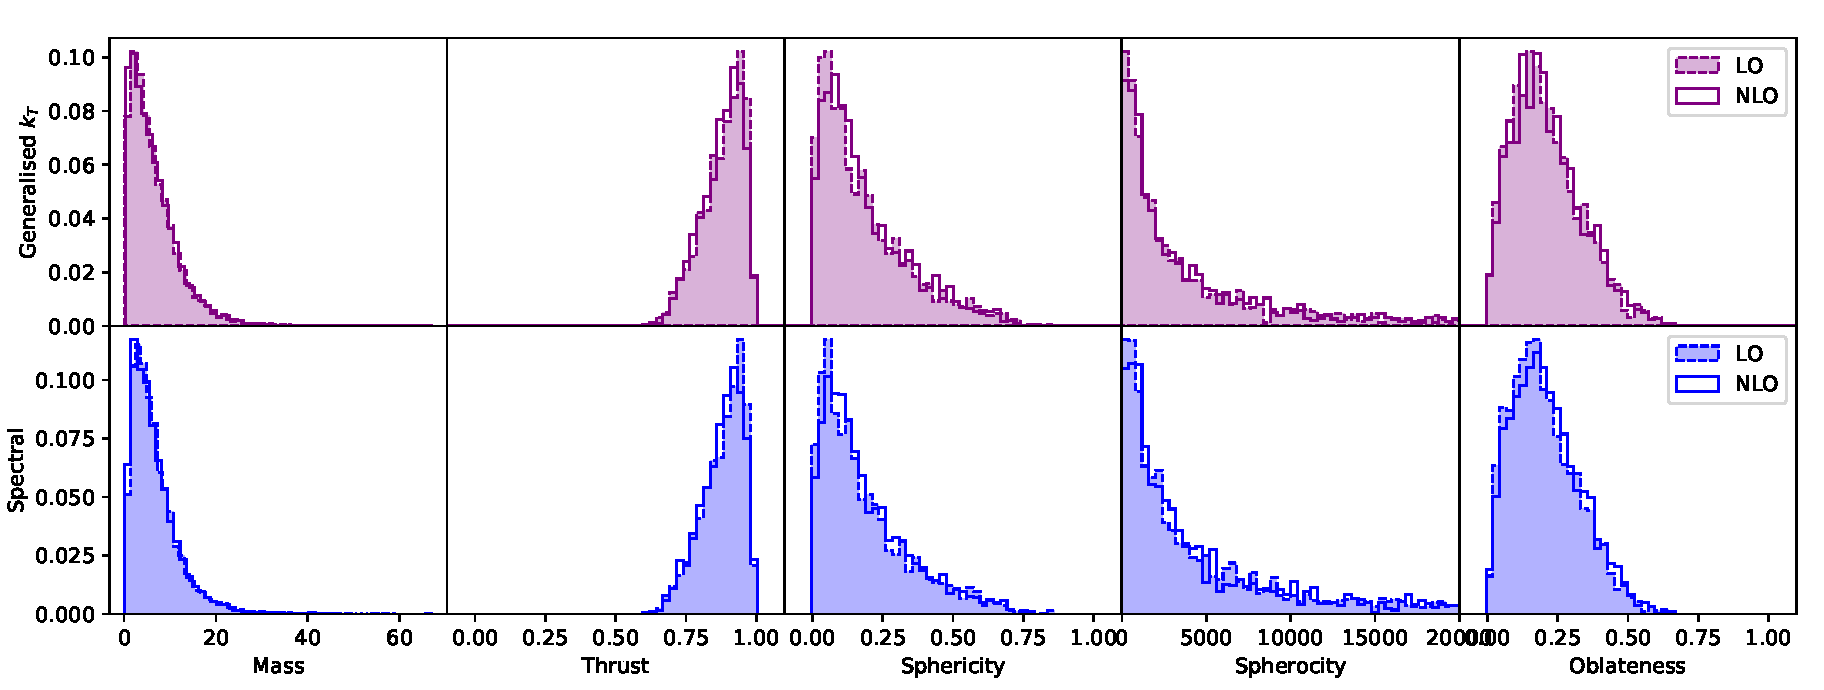
\includegraphics[width=\textwidth]{graphics/array_of_variables2_filled}
    \caption{Spectra for jet properties created with LO and NLO datasets.
             The \(4\) jets with highest \(p_T\) from each event are used in aggregate as an average to 
             form these plots.
             The columns from left to right are: the jet mass, 
             thrust, sphericity, spherocity and oblateness.
             Algorithms where configured (i.e., the settings of \stoppingdeltar{} chosen)
             to give sensible results on
             this dataset, therefore distributions may not represent worst case scenarios.
         }\label{fig:IRC_singles2}
\end{figure}    

However, this method of establishing IR safety only looks at one parameter configuration and could be accused of cherry-picking.
As described in section~\ref{sec:IRmethod}, this can be systematically compared for many parameter configurations by calculating a Jensen-Shannon
score for each LO and NLO pair of jet mass spectra.
If the Jensen-Shannon metric is low, then the two distributions are similar and appear IR safe.
To further clarify the result we include an algorithm known to be IR unsafe, the \itercone{} algorithm, as intimated.
The spectral method produces Jensen-Shannon scores very similar to \genkt{} methods.
Only the iterative cone algorithm produces high Jensen-Shannon scores thus indicating significant changes between the LO and NLO spectra.
This can be seen in Fig.~\ref{fig:unnormedJS}.

\begin{figure}[htp]
    \begin{minipage}[c]{0.5\textwidth}
        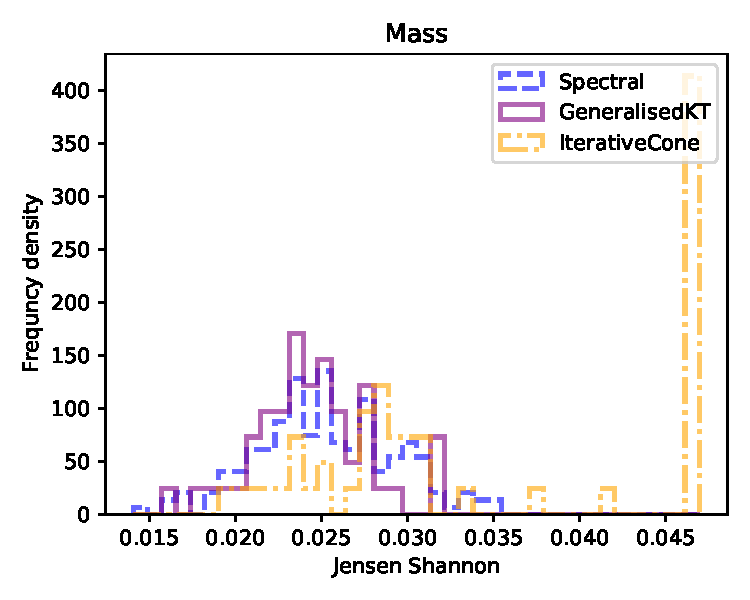
\includegraphics[width=1.\textwidth]{graphics/js_scores/Mass}
    \end{minipage}\hfill
    \begin{minipage}[c]{0.5\textwidth}
        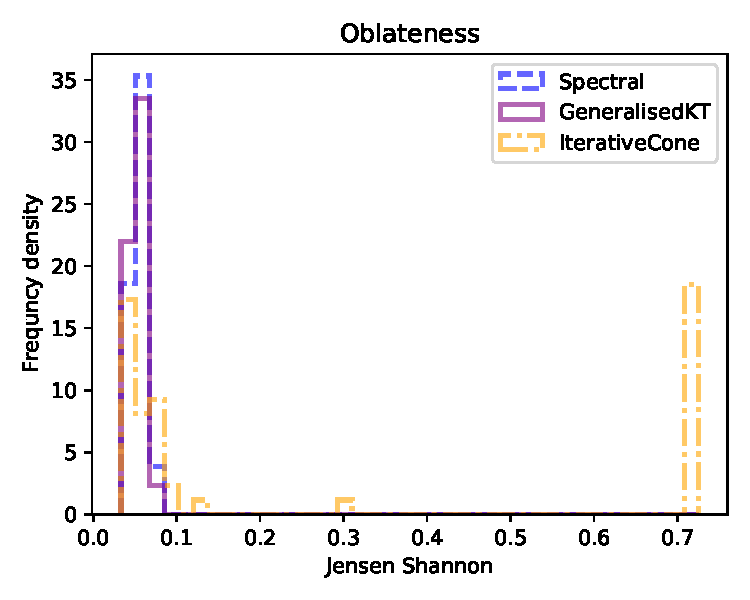
\includegraphics[width=1.\textwidth]{graphics/js_scores/oblateness}
    \end{minipage}
    \begin{minipage}[c]{0.5\textwidth}
        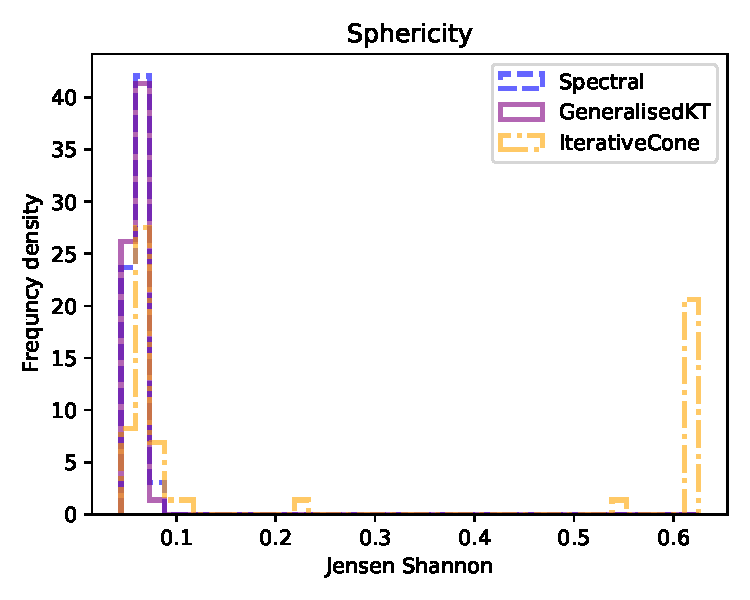
\includegraphics[width=1.\textwidth]{graphics/js_scores/sphericity}
    \end{minipage}\hfill
    \begin{minipage}[c]{0.5\textwidth}
        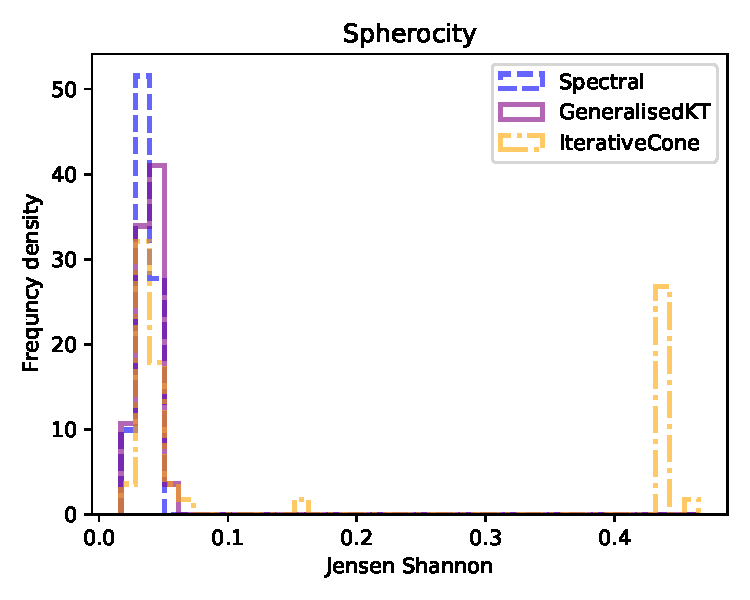
\includegraphics[width=1.\textwidth]{graphics/js_scores/spherocity}
    \end{minipage}
    \begin{minipage}[c]{0.5\textwidth}
        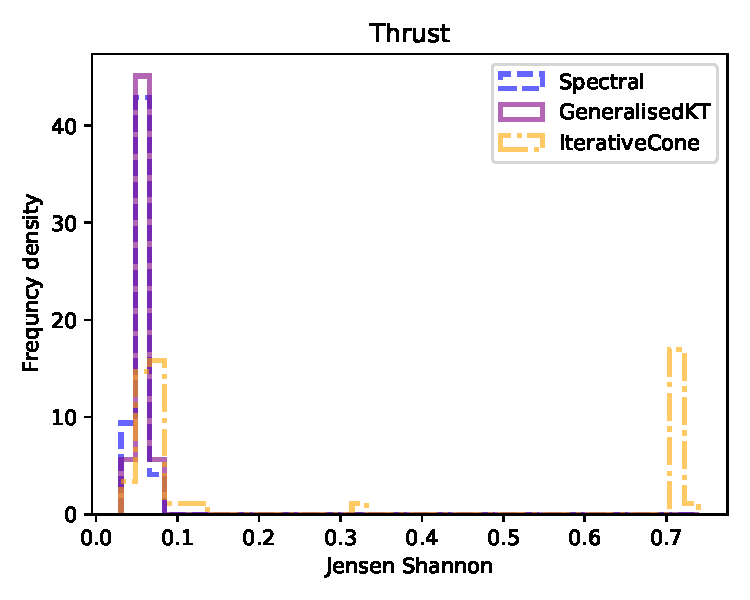
\includegraphics[width=1.\textwidth]{graphics/js_scores/thrust}
    \end{minipage}\hfill
    \begin{minipage}[c]{0.5\textwidth}
    \caption{
        Histograms evaluating IR safety from each jet shape variable.
        Each count is a  Jensen-Shannon score between a probability density of the
        jet shape variable from LO and NLO data.
        Counts at low values indicate insensitivity to IR differences between the LO and NLO data,
        thus IR safety.
     }\label{fig:unnormedJS}
    \end{minipage}
\end{figure}    


From  the last two figures it is clear that \spectral{} clustering  is IR safe, at least, as much as \genkt{} algorithms are.
This contrasts with the \itercone{} algorithm, for which the jet mass spectra at LO and NLO 
differ significantly for many configurations.
This is not unexpected, as the inputs to the \spectral{} clustering algorithm 
are the same as for the Cambridge-Aachen one, 
which is itself IR safe, and the iterative cone has been  proved to produce kinematic configurations which are IR unsafe \cite{Salam:2007xv}.
However, it is crucial to have such a verification in data, as we have done.


\subsection{Mass peak reconstruction}
In this section, the \antikt{} algorithm setups with jet radius \(\ktstoppingdeltar{} = 0.4\) and \(\ktstoppingdeltar{} = 0.8\)
are compared to the \spectral{} algorithm specified in section~\ref{sec:spectralmethodparam}.
The jets are tagged using MC truth.
Each of the \bthing{quarks} created by a signal particle (either a Higgs boson or a top (anti)quark)
tag the closest jet (by using the distance metric \(\sqrt{(y_\text{quark tag} - y_\text{jet})^2 + (\phi_\text{quark tag} - \phi_\text{jet})^2}\)),
provided that the separation between the jet and the quark is no greater than \(0.8\) according to the distance metric.
In the case of a \(W\) decay, the procedure is the same applied to light quark states.
From this point on, only jets tagged this way are considered.


Firstly, jet multiplicities, that is, the number of reconstructed jets found per event, are given for both the anti-$k_T$ and spectral clustering algorithms.
These can be seen for the first three datasets described in section~\ref{sec:particle_data} in Fig.~\ref{fig:multiplicity}. Herein, it
 is seen that \spectral{} clustering produces the best multiplicity (i.e., most events where 4 jets are found) for \underline{Light Higgs} events while for 
         the \underline{Heavy Higgs} and \underline{Top} MC samples  
        it creates a multiplicity closer to that of \antikt{} with \(\ktstoppingdeltar{} = 0.4\) 
        than \(\ktstoppingdeltar{} = 0.8\), the first of these being the best performer of the two. As a result of this study, we remark upon the adaptability of spectral clustering to the different final states without requiring adjusting its parameters, unlike the anti-$k_T$ one. The latter may seem to indicate that 0.4 is the best choice for all datasets, but this is in tension with the fact that different masses from different datasets do require the  anti-$k_T$ algorithm to be adjusted, as we shall now see. 
Mass peaks are constructed from the reconstructed jets as well as, for the top sample only, from the lepton and neutrino.
Again, the \antikt{} results  with \(\stoppingdeltar{}_{k_T} = 0.4\) and \(0.8\) are given for comparison.


\begin{figure}[htp]
    \begin{center}
        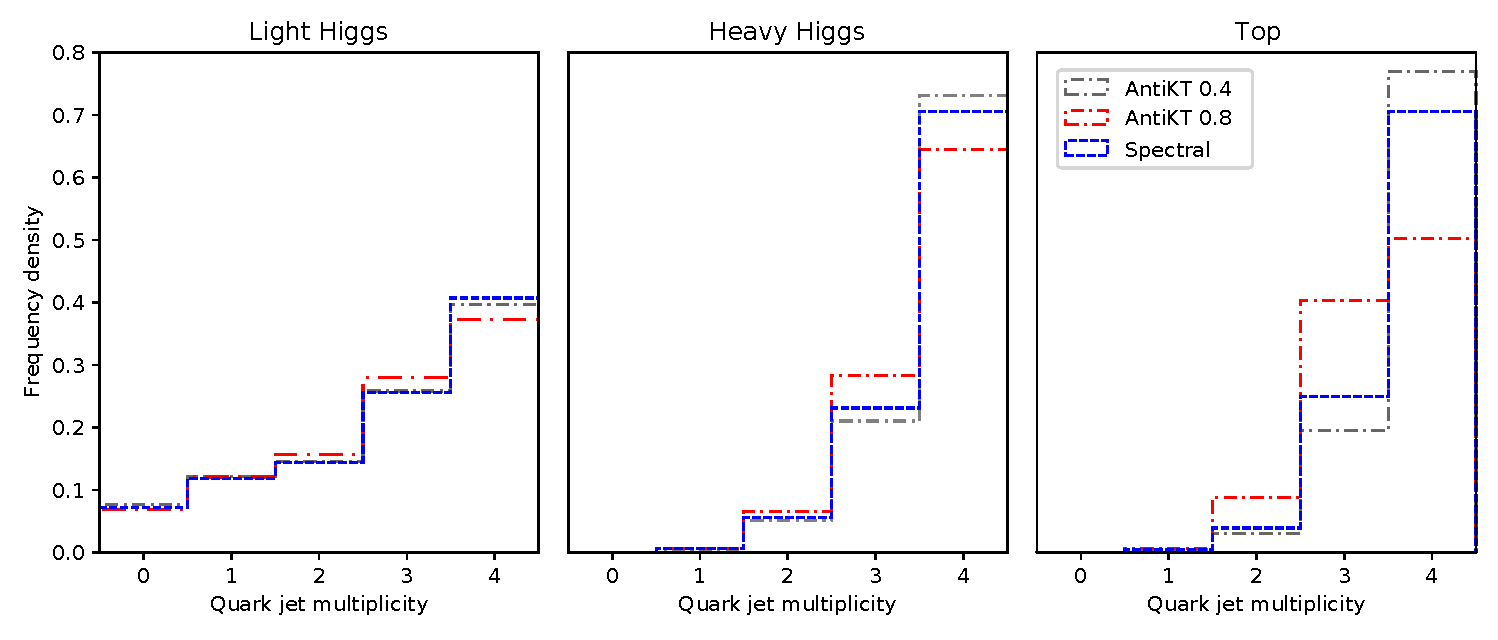
\includegraphics[width=1.0\textwidth]{graphics/multiplicity/multiplicity2}
    \end{center}
    \caption{Jet multiplicities for the anti-$k_T$ (for two jet radius choices) and \spectral{} clustering algorithms on the \underline{Light Higgs}, \underline{Heavy Higgs} and \underline{Top} MC 
 samples. For all such datasets, the hard scattering produces  4 partons in the final  state, so maximising a multiplicity of 4 jets indicates good performance.   
    }\label{fig:multiplicity}
\end{figure}    




In Fig.~\ref{fig:best_correct_h_allocation} three selections are plotted for the \underline{Light Higgs} MC sample. Firstly, we show events where all four \bthing{jets}
are combined for total invariant mass of the event, thus reconstructing the mass of the SM Higgs boson.
Each event also contains two light Higgs states, though. These are differentiated by the mass of the particles (generated by them) that pass the particle cuts,
as follows. The light Higgs boson reconstructed from the $2b$-jet system with more mass visible to the detector is called the ``Light Higgs with stronger signal''
while the one reconstructed  with less mass visible in the detector is called the ``Light Higgs with weaker signal''.
The correct jets for each Higgs mass reconstruction are identified using MC truth,
so the correct pairings are always made. (If two such dijet systems are not found the event is not included in the plots).
Altogether, it can be seen that spectral clustering forms the sharpest peaks and such peaks are all very close to the correct mass. In fact, its performance
is comparable to that of anti-$k_T$ with jet radius 0.8 and is clearly better than the 0.4 option. 


\begin{figure}[htp]
    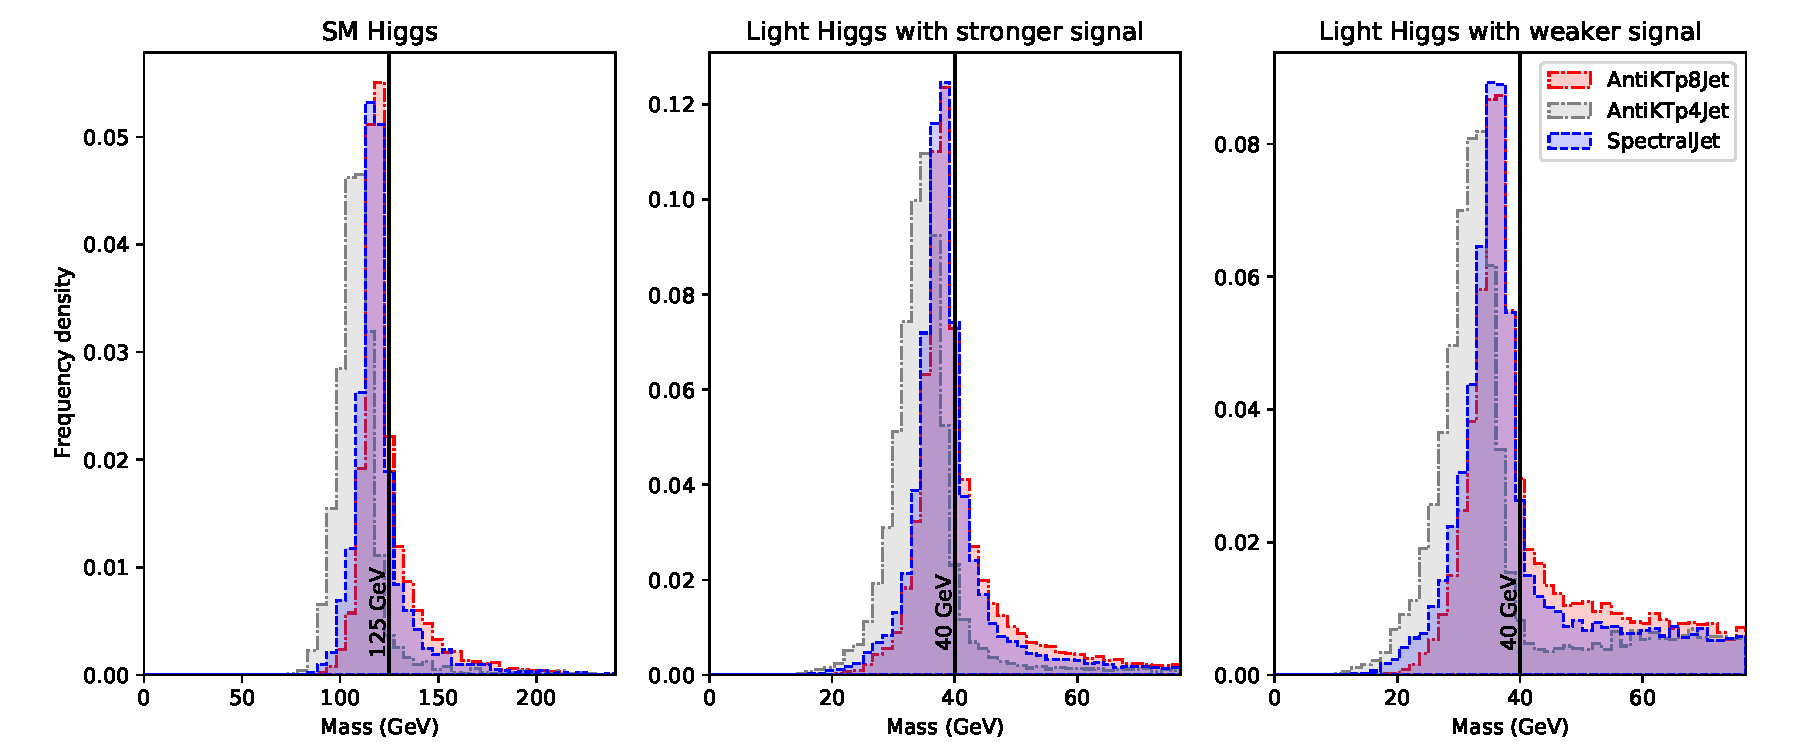
\includegraphics[width=1.\textwidth]{graphics/mass_peaks/light_long_correct_lines.pdf}
    \caption{Three mass selections are plotted for the \underline{Light Higgs} dataset. From left to right we show: the invariant mass of the $4b$-jet system, of the $2b$-jet system with heaviest invariant mass and of the $2b$-jet system with lightest invariant mass (as defined in the text).   Three jet clustering combinations are plotted as detailed in the legend.
        The spectral clustering algorithm is consistently the best performer in terms of the narrowest peaks being reconstructed and comparable to \antikt{} with \(\ktstoppingdeltar{} = 0.8\) in terms of their shift from the true Higgs mass values, with \antikt{} with \(\ktstoppingdeltar{} = 0.4\) always being the outlier. 
    }\label{fig:best_correct_h_allocation}
\end{figure}    

In 
Fig.~\ref{fig:heavy_correct_mass_peaks} the exercise is repeated for the \underline{Heavy Higgs} MC dataset.
All the parameters of \spectral{} clustering are the same as in the \underline{Light Higgs} MC sample yet we note that 
its performance is still excellent, with very sharp peaks at the correct masses, although the three clustering algorithms are overall much closer in performance.
However, recall that, in Fig.~\ref{fig:multiplicity},
it was seen that spectral clustering achieved better multiplicity than \antikt{} with \(\ktstoppingdeltar{} = 0.8\) on this dataset. Furthermore, 
while the multiplicity of \antikt{} with \(\ktstoppingdeltar{} = 0.4\) is a little better, the location of all Higgs mass peaks for \antikt{} with 
\(\ktstoppingdeltar = 0.4\) is slightly worse. So, we are again driven to conclude that spectral clustering is probably the best performer overall with the added benefit of not requiring any adjustment of its parameters to achieve this. 

\begin{figure}[htp]
    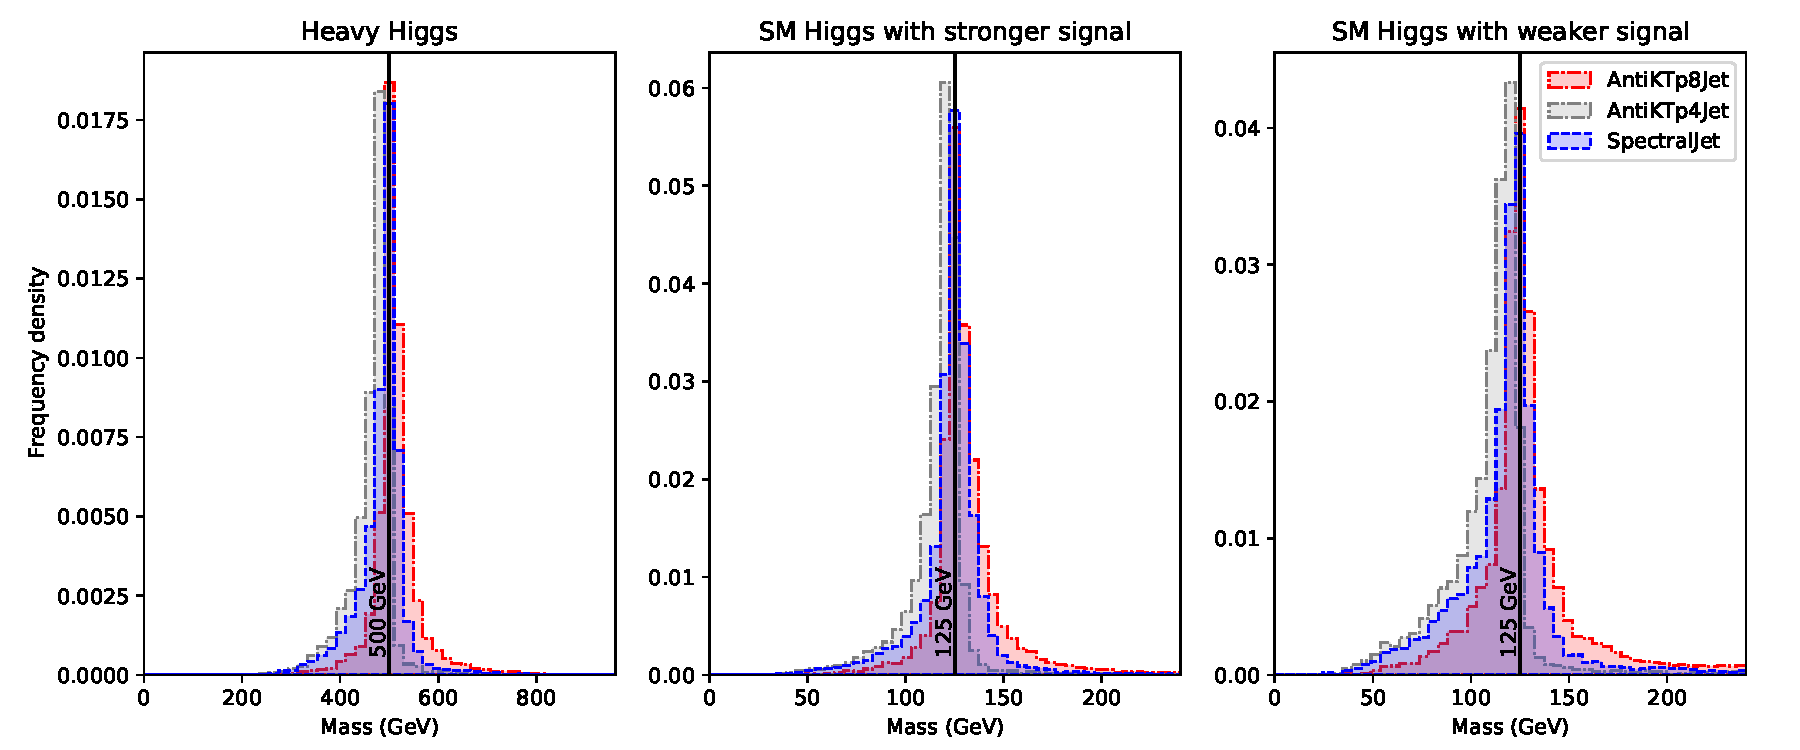
\includegraphics[width=1.\textwidth]{graphics/mass_peaks/heavy_long_correct_lines}
    \caption{Same as Fig.~\ref{fig:best_correct_h_allocation} for the \underline{Heavy Higgs} dataset. Here, the performance of the spectral clustering and \antikt{}
        (with both 0.4 and 0.8 as jet radii) clustering algorithms  is much closer to each other. 
}\label{fig:heavy_correct_mass_peaks}
\end{figure}    


\begin{figure}[htp]
    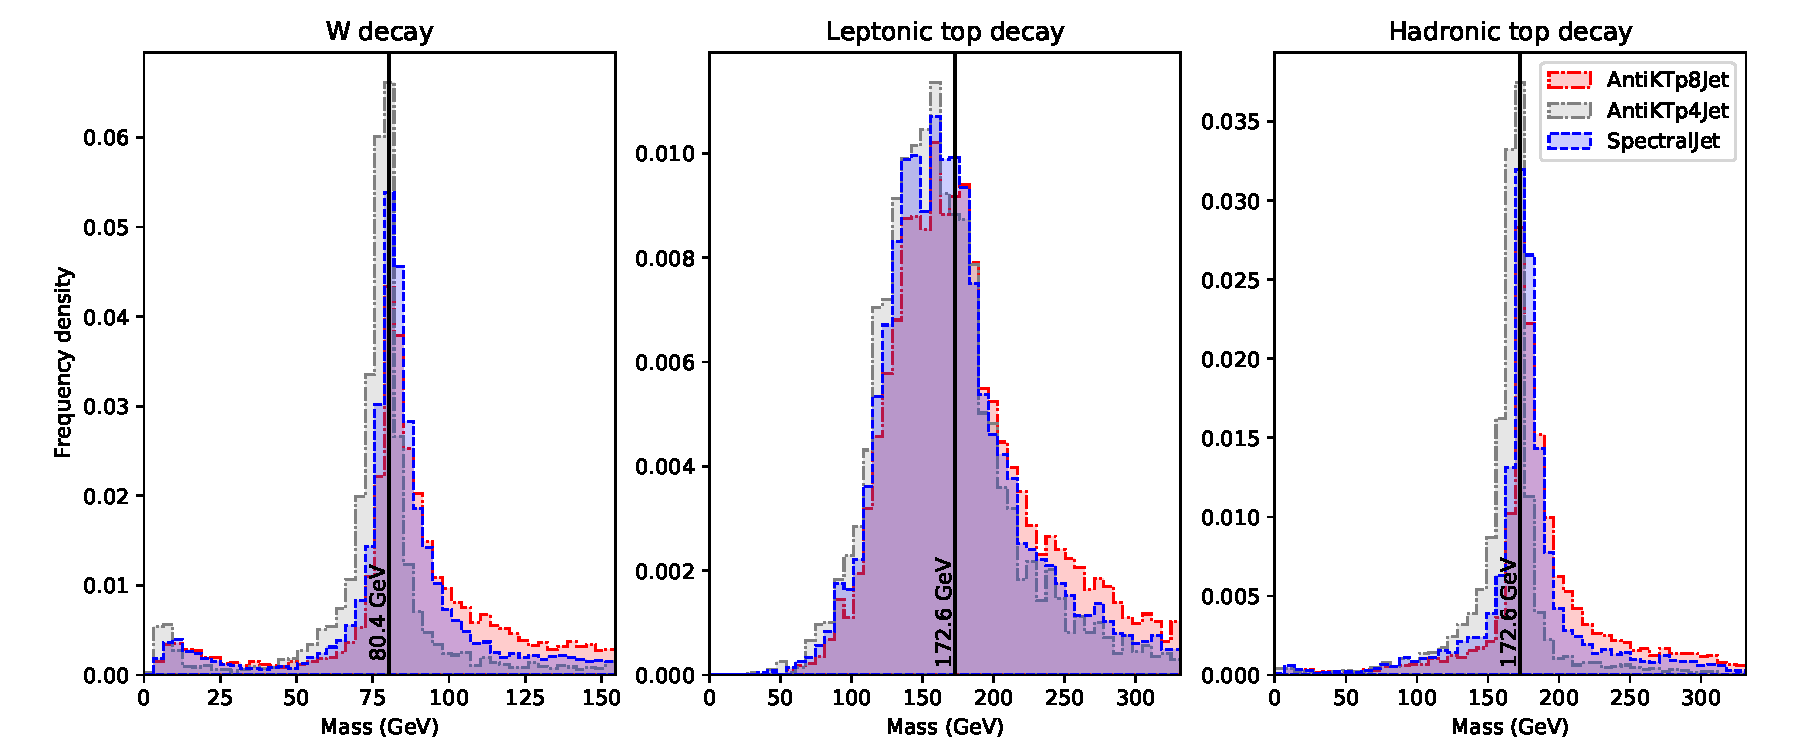
\includegraphics[width=1.\textwidth]{graphics/mass_peaks/top_long_correct_lines}
    \caption{Three mass selections are plotted for the \underline{Top} dataset. From left to right we show: the invariant mass of the light jet system, of the reconstructed leptonic $W$ (as  described in the text) combined with a $b$-jet and of the hadronic $W$ combined with the other $b$-jet. Three jet clustering combinations are plotted as detailed in the legend.
The spectral clustering algorithm  consistently outperforms the  anti-$k_T$ one with jet radius 0.8 and is slightly worse than the anti-$k_T$ one with jet radius 0.4, but only in terms of sharpness, not location.
    }\label{fig:top_correct_mass_peaks}
\end{figure}    

Finally, in Fig.~\ref{fig:top_correct_mass_peaks}, the $W$ and $t$ mass peaks for semileptonic $t\bar t$ decays are shown.
Three mass reconstructions are given.
Firstly, the hadronic \(W\) is reconstructed from the jets that come from the quarks it decayed to.
Correct decisions about which quarks correspond to which particle in the hard process are made by using information in the MC,
this is to prevent any mismatching from causing additional complication in evaluating the performance of the clustering.
To tag a jet with a quark a distance measure \(\sqrt{(y_\text{quark tag} - y_\text{jet})^2 + (\phi_\text{quark tag} - \phi_\text{jet})^2}\)
is used and, if the distance from the quark to the closest jet is less than \(0.8\), that jet is tagged by that quark.
The \(W\) will always decay to a pair of quarks, but both these quarks may be captured in one jet or separate jets.
If either of the these quarks are too far away from the closest jet to tag it,
that is \(\sqrt{(y_\text{quark tag} - y_\text{jet})^2 + (\phi_\text{quark tag} - \phi_\text{jet})^2} > 0.8\),
then it is not associated with any jet and the hadronic \(W\) is not reconstructed.
The mass of the hadronic top is then reconstructed in events where the hadronic \(W\) could be reconstructed and the \bthing{jet}
from the hadronic top is also found.
The leptonic top is then reconstructed in events where a \bthing{jet} from the top is combined with the reconstructed $W$ which as decayed leptonically
The leptonic reconstruction of the $W$ uses the momentum of the electron $p_\ell$, the missing transverse momentum $p_T^{\rm miss}$ (identified with that of the neutrino)
and the longitudinal neutrino momentum ($p_L^\nu$, which is unknown) in a quadratic equation, $(p_\ell+p_T^{\rm miss}+p_L^\nu)^2=m_W^2$, of which only the real solutions are plotted.  In this case, it can be seen that \spectral{} clustering is adapting to jets of a different radius. In fact, 
while before its behaviour had mostly resembled anti-$k_T$ with \(\ktstoppingdeltar{} = 0.8\), 
it has now moved closer to the case with \(\ktstoppingdeltar{} = 0.4\).
(Semileptonic top events would typically be processed using anti-$k_T$ with \(\ktstoppingdeltar{} = 0.4\).)
The peaks of \spectral{} clustering are not quite as narrow as those from anti-$k_T$ with \(\ktstoppingdeltar{} = 0.4\),
but they improve on \(\ktstoppingdeltar{} = 0.8\) and their  location is substantially correct.

